\section{From Parametrized Surface Points to NURBS Representation}
As of yet, there is no open-source software which provides the conversion from a \textit{mesh-based} geometry to NURBS representation. Hence, one of the main challenges of both the algorithmic and implementation part of this project has been to develop one from scratch. Due to a variety of possible approaches to tackle this problem (e.g. \cite{ eck1996automatic, becker2011advanced}), we therefore conducted extensive prototyping work in MATLAB \cite{MATLAB} to avoid cumbersome and time-consuming implementation overheads during the prototyping phase. Once the algorithms to be used had been finalized, the prototypes were implemented a non-proprietary language, Python.

Following the example of using Peters' scheme to fit NURBS smoothly to datapoints in \cite{eck1996automatic}, we did extensive prototyping to ensure the tractability of using Peters' scheme (see \autoref{subsec:peters}) for fitting a NURBS surface (see \autoref{subsub:petersleastsq}) in our settings. As mentioned above, these prototypes were done in MATLAB, and were also partly implemented in Python. 

Incorporated in these algorithms were also the least-squares fitting with a Fairness Functional term (see \autoref{subsec:fairnessthry} and \autoref{subsec:lsqfairness}) to ensure surfaces without unnecessary sharp wiggles.

Among our prototypes for this process we have:
\begin{itemize}
\item A Doo-Sabin subdivision scheme implemented in Python, which we use to organize the twice refined mesh in structures, from which you can extract the locality and neighbour information necessary to calculate the \Bez point coefficients on them in Peters' scheme
\item Implementations of the algorithm to calculate these \Bez point coefficients, as well as plotting them for debugging and visualisation
\item \Bez curve and surface evaluation via calculating the coefficients on each \Bez control point from a set of parameters
\item Algorithms to extract the necessary datapoints and parameters from the result data of the \acf{DC} algorithm in \autoref{ssec:DC}, using geometric conversions where necessary, and ignoring unusual datapoints
\item An algorithm for using the four above algorithms to assemble the total coefficient matrix in \autoref{eqn:petersminimisation} in \autoref{subsub:petersleastsq}
\item An application of MATLAB's built-in least squares minimisation tool to fit the resulting network of \Bez patches to the extracted surface.
\end{itemize}
A sample result, the fitting of a surface to a toroidal shape defined implicitly for the \acs{DC} algorithm is shown in \autoref{fig:fittingStructures}.


\begin{figure}
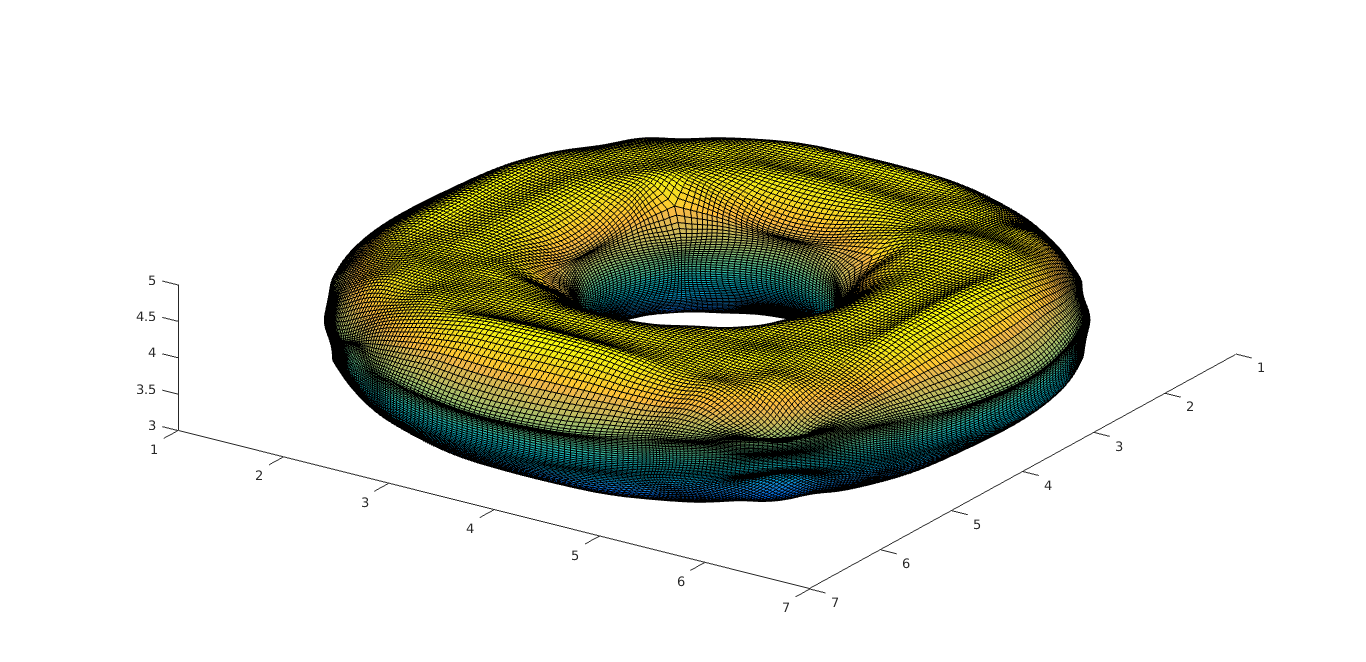
\includegraphics[width = \textwidth]{Pictures/NURBS/torus_from_DC.png}
\caption{A sample result from the Peters' scheme least-squares minimisation surface fitting, using the data provided by the \acs{DC} algorithm for an implicit function describing a torus. The grid lines on the figure are following the constant lines of each parameter value. As they follow the patch edges, corners where other than 4 coarse quads are meeting can be recognized, as for example on the middle of the far side of the torus, on the side that's facing the viewer.}
\label{fig:fittingStructures}
\end{figure}
\todourgent[inline,author=Benni]{From Bezier patches to NURBS using degree elevation. Add this to theory and implementation or only here?}


